\tikzset {_j7xuj04w0/.code = {\pgfsetadditionalshadetransform{ \pgftransformshift{\pgfpoint{0 bp } { 0 bp }  }  \pgftransformrotate{-117 }  \pgftransformscale{2 }  }}}
\pgfdeclarehorizontalshading{_9jgwi88kk}{150bp}{rgb(0bp)=(1,1,1);
    rgb(37.5bp)=(1,1,1);
    rgb(50.08184160505022bp)=(0.95,0.95,0.95);
    rgb(57.64583042689732bp)=(0.88,0.88,0.88);
    rgb(61.33184160505022bp)=(0.96,0.96,0.96);
    rgb(100bp)=(0.96,0.96,0.96)}
\tikzset {_i29mdsrh8/.code = {\pgfsetadditionalshadetransform{ \pgftransformshift{\pgfpoint{0 bp } { 0 bp }  }  \pgftransformrotate{-117 }  \pgftransformscale{2 }  }}}
\pgfdeclarehorizontalshading{_4upvn6zpe}{150bp}{rgb(0bp)=(1,1,1);
    rgb(37.5bp)=(1,1,1);
    rgb(50.08184160505022bp)=(0.95,0.95,0.95);
    rgb(57.64583042689732bp)=(0.88,0.88,0.88);
    rgb(61.33184160505022bp)=(0.96,0.96,0.96);
    rgb(100bp)=(0.96,0.96,0.96)}
\tikzset {_qh2wfjpes/.code = {\pgfsetadditionalshadetransform{ \pgftransformshift{\pgfpoint{0 bp } { 0 bp }  }  \pgftransformrotate{-117 }  \pgftransformscale{2 }  }}}
\pgfdeclarehorizontalshading{_feqyochyi}{150bp}{rgb(0bp)=(1,1,1);
    rgb(37.5bp)=(1,1,1);
    rgb(50.08184160505022bp)=(0.95,0.95,0.95);
    rgb(57.64583042689732bp)=(0.88,0.88,0.88);
    rgb(61.33184160505022bp)=(0.96,0.96,0.96);
    rgb(100bp)=(0.96,0.96,0.96)}
\tikzset {_d10v6gqbc/.code = {\pgfsetadditionalshadetransform{ \pgftransformshift{\pgfpoint{0 bp } { 0 bp }  }  \pgftransformrotate{-117 }  \pgftransformscale{2 }  }}}
\pgfdeclarehorizontalshading{_gk602o946}{150bp}{rgb(0bp)=(1,1,1);
    rgb(37.5bp)=(1,1,1);
    rgb(50.08184160505022bp)=(0.95,0.95,0.95);
    rgb(57.64583042689732bp)=(0.88,0.88,0.88);
    rgb(61.33184160505022bp)=(0.96,0.96,0.96);
    rgb(100bp)=(0.96,0.96,0.96)}
\tikzset {_8lna51u6m/.code = {\pgfsetadditionalshadetransform{ \pgftransformshift{\pgfpoint{0 bp } { 0 bp }  }  \pgftransformrotate{-117 }  \pgftransformscale{2 }  }}}
\pgfdeclarehorizontalshading{_l87ke29nk}{150bp}{rgb(0bp)=(1,1,1);
    rgb(37.5bp)=(1,1,1);
    rgb(50.08184160505022bp)=(0.95,0.95,0.95);
    rgb(57.64583042689732bp)=(0.88,0.88,0.88);
    rgb(61.33184160505022bp)=(0.96,0.96,0.96);
    rgb(100bp)=(0.96,0.96,0.96)}
\tikzset {_flvzdphcz/.code = {\pgfsetadditionalshadetransform{ \pgftransformshift{\pgfpoint{0 bp } { 0 bp }  }  \pgftransformrotate{-117 }  \pgftransformscale{2 }  }}}
\pgfdeclarehorizontalshading{_5rkeipgwd}{150bp}{rgb(0bp)=(1,1,1);
    rgb(37.5bp)=(1,1,1);
    rgb(50.08184160505022bp)=(0.95,0.95,0.95);
    rgb(57.64583042689732bp)=(0.88,0.88,0.88);
    rgb(61.33184160505022bp)=(0.96,0.96,0.96);
    rgb(100bp)=(0.96,0.96,0.96)}
\tikzset {_lvfzf5nu3/.code = {\pgfsetadditionalshadetransform{ \pgftransformshift{\pgfpoint{0 bp } { 0 bp }  }  \pgftransformrotate{-117 }  \pgftransformscale{2 }  }}}
\pgfdeclarehorizontalshading{_65i61e978}{150bp}{rgb(0bp)=(1,1,1);
    rgb(37.5bp)=(1,1,1);
    rgb(50.08184160505022bp)=(0.95,0.95,0.95);
    rgb(57.64583042689732bp)=(0.88,0.88,0.88);
    rgb(61.33184160505022bp)=(0.96,0.96,0.96);
    rgb(100bp)=(0.96,0.96,0.96)}
\tikzset {_27lop19l0/.code = {\pgfsetadditionalshadetransform{ \pgftransformshift{\pgfpoint{0 bp } { 0 bp }  }  \pgftransformrotate{-117 }  \pgftransformscale{2 }  }}}
\pgfdeclarehorizontalshading{_h3pg9rf15}{150bp}{rgb(0bp)=(1,1,1);
    rgb(37.5bp)=(1,1,1);
    rgb(50.08184160505022bp)=(0.95,0.95,0.95);
    rgb(57.64583042689732bp)=(0.88,0.88,0.88);
    rgb(61.33184160505022bp)=(0.96,0.96,0.96);
    rgb(100bp)=(0.96,0.96,0.96)}
\tikzset {_3yz7x95el/.code = {\pgfsetadditionalshadetransform{ \pgftransformshift{\pgfpoint{0 bp } { 0 bp }  }  \pgftransformrotate{-117 }  \pgftransformscale{2 }  }}}
\pgfdeclarehorizontalshading{_Ae1dgwonr}{150bp}{rgb(0bp)=(1,1,1);
    rgb(37.5bp)=(1,1,1);
    rgb(50.08184160505022bp)=(0.95,0.95,0.95);
    rgb(57.64583042689732bp)=(0.88,0.88,0.88);
    rgb(61.33184160505022bp)=(0.96,0.96,0.96);
    rgb(100bp)=(0.96,0.96,0.96)}
\tikzset {_hfu6x8eun/.code = {\pgfsetadditionalshadetransform{ \pgftransformshift{\pgfpoint{0 bp } { 0 bp }  }  \pgftransformrotate{-117 }  \pgftransformscale{2 }  }}}
\pgfdeclarehorizontalshading{_titklq3j6}{150bp}{rgb(0bp)=(1,1,1);
    rgb(37.5bp)=(1,1,1);
    rgb(50.08184160505022bp)=(0.95,0.95,0.95);
    rgb(57.64583042689732bp)=(0.88,0.88,0.88);
    rgb(61.33184160505022bp)=(0.96,0.96,0.96);
    rgb(100bp)=(0.96,0.96,0.96)}
\tikzset{every picture/.style={line width=0.75pt}}
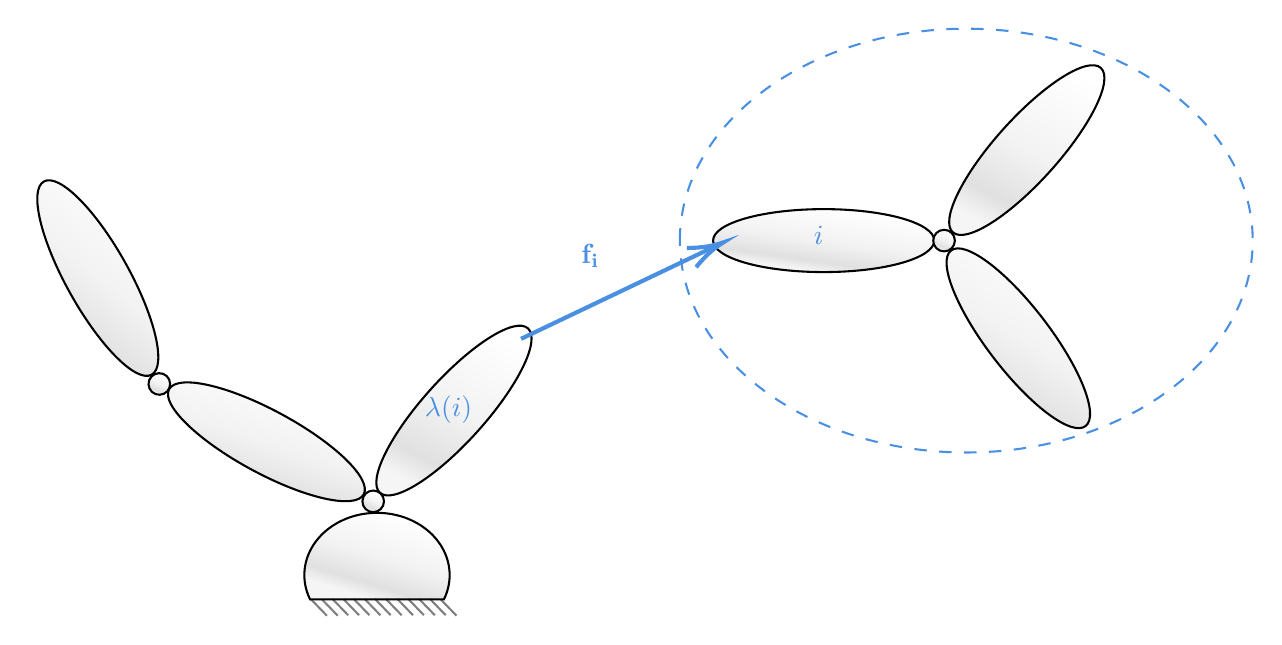
\begin{tikzpicture}[x=0.75pt,y=0.75pt,yscale=-1,xscale=1]
    \path  [shading=_9jgwi88kk,_j7xuj04w0] (382.42,149.33) .. controls (382.42,140.96) and (406.28,134.17) .. (435.71,134.17) .. controls (465.14,134.17) and (489,140.96) .. (489,149.33) .. controls (489,157.71) and (465.14,164.5) .. (435.71,164.5) .. controls (406.28,164.5) and (382.42,157.71) .. (382.42,149.33) -- cycle ;
    \draw  [color={rgb, 255:red, 0; green, 0; blue, 0 }  ,draw opacity=1 ][line width=0.75]  (382.42,149.33) .. controls (382.42,140.96) and (406.28,134.17) .. (435.71,134.17) .. controls (465.14,134.17) and (489,140.96) .. (489,149.33) .. controls (489,157.71) and (465.14,164.5) .. (435.71,164.5) .. controls (406.28,164.5) and (382.42,157.71) .. (382.42,149.33) -- cycle ;
    \path  [shading=_4upvn6zpe,_i29mdsrh8] (569.22,66.11) .. controls (575.45,71.72) and (564.53,93.99) .. (544.84,115.87) .. controls (525.15,137.75) and (504.14,150.94) .. (497.92,145.33) .. controls (491.69,139.73) and (502.61,117.45) .. (522.3,95.58) .. controls (541.99,73.7) and (563,60.51) .. (569.22,66.11) -- cycle ;
    \draw  [color={rgb, 255:red, 0; green, 0; blue, 0 }  ,draw opacity=1 ][line width=0.75]  (569.22,66.11) .. controls (575.45,71.72) and (564.53,93.99) .. (544.84,115.87) .. controls (525.15,137.75) and (504.14,150.94) .. (497.92,145.33) .. controls (491.69,139.73) and (502.61,117.45) .. (522.3,95.58) .. controls (541.99,73.7) and (563,60.51) .. (569.22,66.11) -- cycle ;
    \path  [shading=_feqyochyi,_qh2wfjpes] (488.5,149.33) .. controls (488.5,146.46) and (490.83,144.13) .. (493.71,144.13) .. controls (496.58,144.13) and (498.92,146.46) .. (498.92,149.33) .. controls (498.92,152.21) and (496.58,154.54) .. (493.71,154.54) .. controls (490.83,154.54) and (488.5,152.21) .. (488.5,149.33) -- cycle ;
    \draw  [color={rgb, 255:red, 0; green, 0; blue, 0 }  ,draw opacity=1 ][line width=0.75]  (488.5,149.33) .. controls (488.5,146.46) and (490.83,144.13) .. (493.71,144.13) .. controls (496.58,144.13) and (498.92,146.46) .. (498.92,149.33) .. controls (498.92,152.21) and (496.58,154.54) .. (493.71,154.54) .. controls (490.83,154.54) and (488.5,152.21) .. (488.5,149.33) -- cycle ;
    \path  [shading=_gk602o946,_d10v6gqbc] (293.22,191.61) .. controls (299.45,197.22) and (288.53,219.49) .. (268.84,241.37) .. controls (249.15,263.25) and (228.14,276.44) .. (221.92,270.83) .. controls (215.69,265.23) and (226.61,242.95) .. (246.3,221.08) .. controls (265.99,199.2) and (287,186.01) .. (293.22,191.61) -- cycle ;
    \draw  [color={rgb, 255:red, 0; green, 0; blue, 0 }  ,draw opacity=1 ][line width=0.75]  (293.22,191.61) .. controls (299.45,197.22) and (288.53,219.49) .. (268.84,241.37) .. controls (249.15,263.25) and (228.14,276.44) .. (221.92,270.83) .. controls (215.69,265.23) and (226.61,242.95) .. (246.3,221.08) .. controls (265.99,199.2) and (287,186.01) .. (293.22,191.61) -- cycle ;
    \path  [shading=_l87ke29nk,_8lna51u6m] (213.46,274.96) .. controls (213.46,272.08) and (215.79,269.75) .. (218.67,269.75) .. controls (221.54,269.75) and (223.87,272.08) .. (223.87,274.96) .. controls (223.87,277.83) and (221.54,280.17) .. (218.67,280.17) .. controls (215.79,280.17) and (213.46,277.83) .. (213.46,274.96) -- cycle ;
    \draw  [color={rgb, 255:red, 0; green, 0; blue, 0 }  ,draw opacity=1 ][line width=0.75]  (213.46,274.96) .. controls (213.46,272.08) and (215.79,269.75) .. (218.67,269.75) .. controls (221.54,269.75) and (223.87,272.08) .. (223.87,274.96) .. controls (223.87,277.83) and (221.54,280.17) .. (218.67,280.17) .. controls (215.79,280.17) and (213.46,277.83) .. (213.46,274.96) -- cycle ;
    \path  [shading=_5rkeipgwd,_flvzdphcz] (111.95,213.93) .. controls (104.63,218.01) and (87.08,200.48) .. (72.74,174.78) .. controls (58.4,149.08) and (52.7,124.93) .. (60.02,120.85) .. controls (67.33,116.77) and (84.89,134.3) .. (99.23,160) .. controls (113.57,185.7) and (119.26,209.85) .. (111.95,213.93) -- cycle ;
    \draw  [color={rgb, 255:red, 0; green, 0; blue, 0 }  ,draw opacity=1 ][line width=0.75]  (111.95,213.93) .. controls (104.63,218.01) and (87.08,200.48) .. (72.74,174.78) .. controls (58.4,149.08) and (52.7,124.93) .. (60.02,120.85) .. controls (67.33,116.77) and (84.89,134.3) .. (99.23,160) .. controls (113.57,185.7) and (119.26,209.85) .. (111.95,213.93) -- cycle ;
    \path  [shading=_65i61e978,_lvfzf5nu3] (120.33,220.95) .. controls (124.31,213.58) and (148.53,218.94) .. (174.43,232.93) .. controls (200.32,246.91) and (218.09,264.22) .. (214.11,271.59) .. controls (210.13,278.96) and (185.91,273.6) .. (160.01,259.62) .. controls (134.12,245.63) and (116.35,228.32) .. (120.33,220.95) -- cycle ;
    \draw  [color={rgb, 255:red, 0; green, 0; blue, 0 }  ,draw opacity=1 ][line width=0.75]  (120.33,220.95) .. controls (124.31,213.58) and (148.53,218.94) .. (174.43,232.93) .. controls (200.32,246.91) and (218.09,264.22) .. (214.11,271.59) .. controls (210.13,278.96) and (185.91,273.6) .. (160.01,259.62) .. controls (134.12,245.63) and (116.35,228.32) .. (120.33,220.95) -- cycle ;
    \path  [shading=_h3pg9rf15,_27lop19l0] (115.79,223.61) .. controls (112.92,223.71) and (110.51,221.45) .. (110.42,218.58) .. controls (110.32,215.7) and (112.58,213.3) .. (115.45,213.2) .. controls (118.33,213.11) and (120.73,215.36) .. (120.83,218.24) .. controls (120.92,221.11) and (118.67,223.52) .. (115.79,223.61) -- cycle ;
    \draw  [color={rgb, 255:red, 0; green, 0; blue, 0 }  ,draw opacity=1 ][line width=0.75]  (115.79,223.61) .. controls (112.92,223.71) and (110.51,221.45) .. (110.42,218.58) .. controls (110.32,215.7) and (112.58,213.3) .. (115.45,213.2) .. controls (118.33,213.11) and (120.73,215.36) .. (120.83,218.24) .. controls (120.92,221.11) and (118.67,223.52) .. (115.79,223.61) -- cycle ;
    \path  [shading=_Ae1dgwonr,_3yz7x95el] (561.88,238.7) .. controls (555.23,243.8) and (535.33,228.98) .. (517.44,205.61) .. controls (499.55,182.24) and (490.43,159.17) .. (497.09,154.08) .. controls (503.74,148.98) and (523.63,163.8) .. (541.53,187.17) .. controls (559.42,210.54) and (568.53,233.61) .. (561.88,238.7) -- cycle ;
    \draw  [color={rgb, 255:red, 0; green, 0; blue, 0 }  ,draw opacity=1 ][line width=0.75]  (561.88,238.7) .. controls (555.23,243.8) and (535.33,228.98) .. (517.44,205.61) .. controls (499.55,182.24) and (490.43,159.17) .. (497.09,154.08) .. controls (503.74,148.98) and (523.63,163.8) .. (541.53,187.17) .. controls (559.42,210.54) and (568.53,233.61) .. (561.88,238.7) -- cycle ;
    \draw [color={rgb, 255:red, 74; green, 144; blue, 226 }  ,draw opacity=1 ][line width=1.5]    (289.92,196.67) -- (384.71,151.46) ;
    \draw [shift={(387.42,150.17)}, rotate = 154.5] [color={rgb, 255:red, 74; green, 144; blue, 226 }  ,draw opacity=1 ][line width=1.5]    (17.05,-5.13) .. controls (10.84,-2.18) and (5.16,-0.47) .. (0,0) .. controls (5.16,0.47) and (10.84,2.18) .. (17.05,5.13)   ;
    \draw  [color={rgb, 255:red, 74; green, 144; blue, 226 }  ,draw opacity=1 ][dash pattern={on 4.5pt off 4.5pt}] (366.42,149.33) .. controls (366.42,92.95) and (428.2,47.25) .. (504.42,47.25) .. controls (580.63,47.25) and (642.42,92.95) .. (642.42,149.33) .. controls (642.42,205.71) and (580.63,251.42) .. (504.42,251.42) .. controls (428.2,251.42) and (366.42,205.71) .. (366.42,149.33) -- cycle ;
    \path  [shading=_titklq3j6,_hfu6x8eun] (188.28,322.23) .. controls (186.49,318.63) and (185.5,314.66) .. (185.5,310.5) .. controls (185.5,293.93) and (201.17,280.5) .. (220.5,280.5) .. controls (239.83,280.5) and (255.5,293.93) .. (255.5,310.5) .. controls (255.5,314.66) and (254.51,318.63) .. (252.72,322.23) -- cycle ;
    \draw   (188.28,322.23) .. controls (186.49,318.63) and (185.5,314.66) .. (185.5,310.5) .. controls (185.5,293.93) and (201.17,280.5) .. (220.5,280.5) .. controls (239.83,280.5) and (255.5,293.93) .. (255.5,310.5) .. controls (255.5,314.66) and (254.51,318.63) .. (252.72,322.23) -- cycle ;
    \draw [color={rgb, 255:red, 0; green, 0; blue, 0 }  ,draw opacity=0.5 ]   (188.78,322.23) -- (196.36,330.06) ;
    \draw [color={rgb, 255:red, 0; green, 0; blue, 0 }  ,draw opacity=0.5 ]   (251.22,322.23) -- (258.81,330.06) ;
    \draw [color={rgb, 255:red, 0; green, 0; blue, 0 }  ,draw opacity=0.5 ]   (194.03,322.23) -- (201.61,330.06) ;
    \draw [color={rgb, 255:red, 0; green, 0; blue, 0 }  ,draw opacity=0.5 ]   (199.03,321.98) -- (206.61,329.81) ;
    \draw [color={rgb, 255:red, 0; green, 0; blue, 0 }  ,draw opacity=0.5 ]   (204.28,321.98) -- (211.86,329.81) ;
    \draw [color={rgb, 255:red, 0; green, 0; blue, 0 }  ,draw opacity=0.5 ]   (209.28,321.98) -- (216.86,329.81) ;
    \draw [color={rgb, 255:red, 0; green, 0; blue, 0 }  ,draw opacity=0.5 ]   (214.53,321.98) -- (222.11,329.81) ;
    \draw [color={rgb, 255:red, 0; green, 0; blue, 0 }  ,draw opacity=0.5 ]   (219.53,321.98) -- (227.11,329.81) ;
    \draw [color={rgb, 255:red, 0; green, 0; blue, 0 }  ,draw opacity=0.5 ]   (224.78,321.98) -- (232.36,329.81) ;
    \draw [color={rgb, 255:red, 0; green, 0; blue, 0 }  ,draw opacity=0.5 ]   (230.28,321.98) -- (237.86,329.81) ;
    \draw [color={rgb, 255:red, 0; green, 0; blue, 0 }  ,draw opacity=0.5 ]   (235.53,321.98) -- (243.11,329.81) ;
    \draw [color={rgb, 255:red, 0; green, 0; blue, 0 }  ,draw opacity=0.5 ]   (240.78,321.98) -- (248.36,329.81) ;
    \draw [color={rgb, 255:red, 0; green, 0; blue, 0 }  ,draw opacity=0.5 ]   (246.03,321.98) -- (253.61,329.81) ;
    \draw (317.5,149.4) node [anchor=north west][inner sep=0.75pt]  [color={rgb, 255:red, 74; green, 144; blue, 226 }  ,opacity=1 ]  {${\displaystyle \mathbf{f_{i}}}$};
    \draw (429.5,140.9) node [anchor=north west][inner sep=0.75pt]    {$\textcolor[rgb]{0.29,0.56,0.89}{i}$};
    \draw  [draw opacity=0]  (256.6, 230.8) circle [x radius= 21.92, y radius= 14.85]   ;
    \draw (242.1,222.7) node [anchor=north west][inner sep=0.75pt]    {$\textcolor[rgb]{0.29,0.56,0.89}{\lambda }\textcolor[rgb]{0.29,0.56,0.89}{(}\textcolor[rgb]{0.29,0.56,0.89}{i}\textcolor[rgb]{0.29,0.56,0.89}{)}$};
\end{tikzpicture}